\documentclass{article}
\usepackage{amsmath, array, graphicx}
\title{Bespoke splines}
\author{Raph Levien}
\date{\today}

\newcommand{\kcurve}{$\kappa$-Curve}

\begin{document}
\maketitle

\begin{abstract}
The quest for better splines for interactive curve design continues. The Euler spiral spline has a long tradition and is very fine when bending angles in the control polygon are small, but does not have a unique stable solution when angles increase. A new analysis shows that the family of ``two parameter splines'' can encompass a wide range of desirable behavior based on properties of a 2-dimensional curvature map. In particular, a periodic curvature map can yield robust splines, so a perturbation of the control points changes the resulting curve only slightly. This paper proposes a new spline that is robust over all inputs and preserves much of the quality of the Euler spiral spline. This spline is but one instance of a powerful design methodology that can produce splines optimizing for specific desired properties, based on the two-parameter paradigm.
\end{abstract}

\section{Introduction}

Tools for interactive curve design still feel primitive, in spite of much work on interpolating splines. Most professional curve design work, including font design, is done using B{\'e}zier curves. Such curves are difficult to learn and require expert operation to produce smooth results. Yet, they are expressive, and feel very robust in interactive use, so they remain.

One of the oldest and most promising splines for interactive use is the Euler spiral spline. With gentle inputs (no sharp bending angles), it produces very fine results. But in interactive exploration, for example when sketching new ideas, it's not hard to put the spline into a state where loops suddenly flip direction. Some implementations, fail to converge entirely, as Newton-based solvers are not always well conditioned. The author's own Spiro implementation, which includes Euler spiral splines, occasionally produces curves resembling particle accelerator tracks when the solver fails.

Recently Adobe has proposed a new spline \cite{Yan:2017:KCI:3072959.3073692} which solves the robustness problem, but at the cost of lumpier results than the Euler spiral spline. The main theme of this paper is to explore the obvious question of whether it is somehow possible to combine the best features of both.

\subsection{What is the best spline?}

It would be nice to design a perfect spline, but such a thing is not possible. Instead, there are a number of properties of splines, and it is possible to optimize for a subset. A fairly thorough listing of such properties is given in Chapter 2 of my thesis \cite{Lev09}. In some cases, these properties are in direct conflict with each other.

Take \emph{roundness} for example, the property that three points in a cyclic configuration will form the unique circle through those three points (and, more generally, the tendency of the spline to generate circular arcs). This seems like one of the most basic and desirable properties of a spline, but a round spline sacrifices \emph{boundedness} and \emph{robustness,} as can be seen when the points pass through a co-linear configuration; the circle goes through an infinite radius.

Even so, listing desirable properties provides scant help in actually designing a spline. The space of all possible splines is vast -- for any sequence of control points, it produces a curve (an infinite-dimensional class of objects) constrained only by the requirement to interpolate the control points. Is there some discipline that can reduce this space to something tractable to reason about, preserving the ``good'' splines? I argue below that the \emph{two parameter paradigm} is exactly such a discipline.

\section{Two parameter splines}

Chapter 4 of my thesis \cite{Lev09} proposed a framework of \emph{two parameter splines.} In this framework a family of curves to be instantiated at each segment between to control points, parametrized by the tangent angles at each endpoint relative to the chord. The segment is rotated and scaled in place so the endpoints of the segment match the control points.

In this framework, the tangents at each control point are free parameters (there is only one tangent for each control point, as G1 continuity is by construction). The spline then solves these parameters for G2 continuity at each control point.

Note that in this framework, the assignment of tangents depends only on the curvature at the endpoint of each segment, which in turn is a function of the two parameters. In this way, it \emph{decouples} the shape of the segments from the global behavior of the spline. Two curve families with the same \emph{curvature map} will be assigned the same tangents even if the interior shapes differ.

The loose coupling is emphasized even more if there is a four-parameter curve family that can fit arbitrary tangent and curvature constraints at both endpoints. With such a family, any curvature map can be accommodated.

The most familiar example of such a four-parameter family is a cubic B{\'e}zier. Other examples include 4th order polynomial spirals (Spiro curves), or quintic B{\'e}zier curves constrained to have nearly constant velocity.

\subsection{Existing 2-parameter splines}

A number of existing splines into the literature fit into the 2-parameter framework. In many cases, such splines are optimized for some property, providing evidence for the proposition that by choosing a 2-parameter curve family based on some property, the spline is globally optimized for this property.

Perhaps the most striking example is the Minimum Energy Curve (MEC). Defining a 2-parameter curve family minimizing the bending energy of a thin strip of flexible material passing through the endpoints with the given tangent constraints, the resulting spline globally minimizes bending energy for all curves passing through the control points.

The MEC has a number of drawbacks; most notably it tends to produce curves of lower tension (longer length) than intuitively desirable, as bending energy scales inversely with curve length. Of the approaches to increase tension, perhaps the most effective is the Euler spiral spline, which fits segments of the Euler spiral, or, equivalently, defines curve segments as having curvature linear in arclength. The resulting splines are quite pleasing and have a number of desirable properties, but also a significant drawback: at large bending angles, there is not a unique solution, and a solver tends to ``flip'' suddenly from one configuration to another, even for small perturbations of the control points. This is likely a major reason Euler spliral splines have not been adopted more widely (certainly as argued by Yan et al \cite{Yan:2017:KCI:3072959.3073692}).

The curvature map of the Euler spiral is shown in Figure \ref{euler_kmap}. For this region of the parameter space (angles between $-\pi/2$ and $\pi/2$), it is very smooth, almost linear, and curvature is bounded.

\begin{figure}
\centering
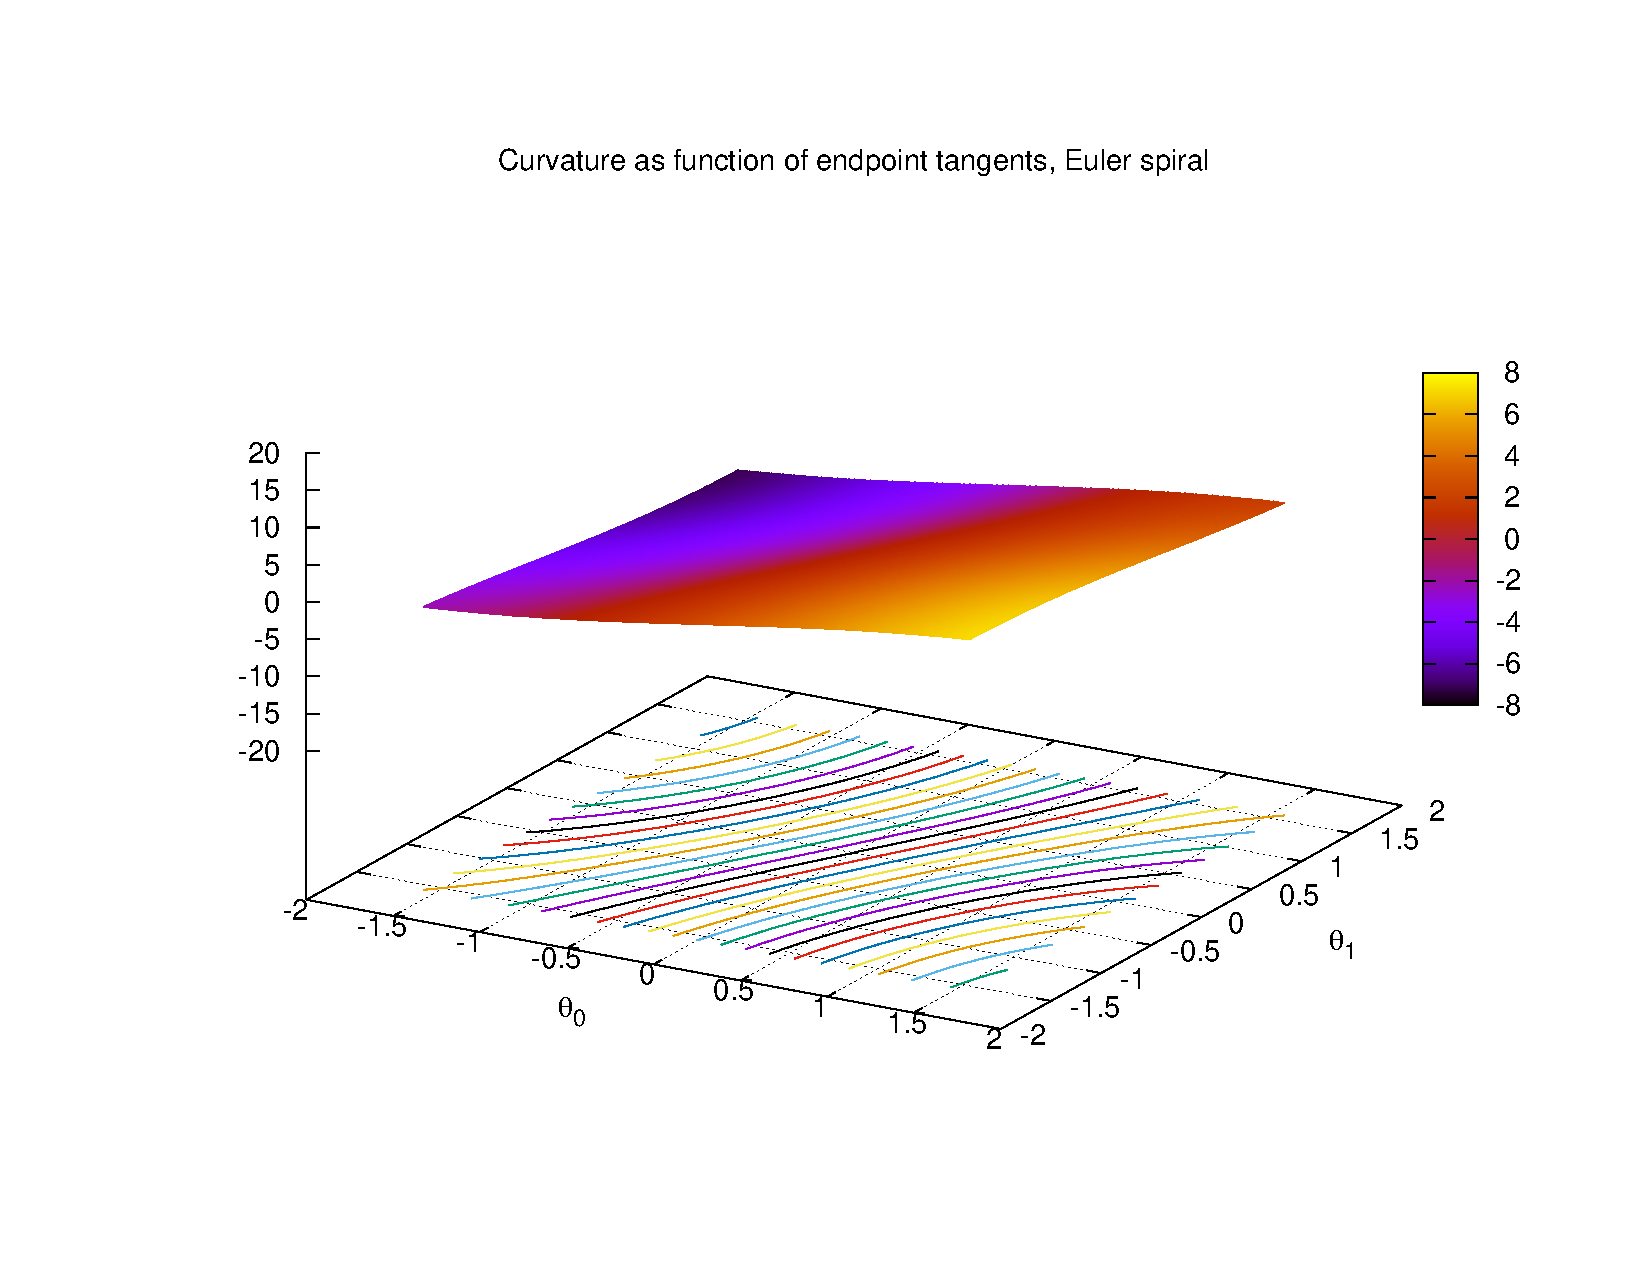
\includegraphics[scale=0.5]{euler_kmap}
\caption{Curvature map of Euler spiral}
\label{euler_kmap}
\end{figure}

Both MEC and Euler spiral splines are \emph{extensional,} meaning that refining a spline by placing an additional control point on the curve does not change the spline. As my thesis explains, extensional 2-parameter splines are quite restricted; all curves must be sections of a fixed generating curve.

Another spline that fits into the two-parameter framework is the \emph{circle spline} of S{\'e}quin et al \cite{DBLP:journals/cad/SequinLY05}. In this spline, the curvature at an endpoint is fixed as that of the unique circle passing through the tangent constraint at that endpoint and intersecting the other endpoint. Circle splines have excellent \emph{locality} but fails extensionality quite dramatically (producing particularly lumpy results when placing a new point near an inflection).


\subsection{Analysis of \kcurve{}s in 2-parameter framework}

With a bit of insight, it can be seen that the 2-parameter framework is general enough to include the \kcurve{} spline. In this analysis, the curve family consists of two parabola segments, with the vertex of each parabola at the endpoint, and the (absolute) curvature matched at the join point. This can be called a ``bi-parabola'' in analogy to the ``biarc'' as used in the Ikarus system \cite{Karow87}. Solving for G2 continuity at control points produces a single parabola segment that spans both sides of each control point (there is a unique parabola of given tangent and curvature at the vertex). This is true even if the interiors of segments in the curve family are not G2 continuous, as is the case for in the pseudo-inflectional case where the endpoints have curvature of opposite sign.

The construction of a bi-parabola from tangent constraints is shown in Figure \ref{biparabola}. For any pair of tangent constraints, there is a unique pair of parabolas with vertex at the endpoints, going through the tangents, and meeting at a point of equal curvature magnitude.

\begin{figure}
\centering
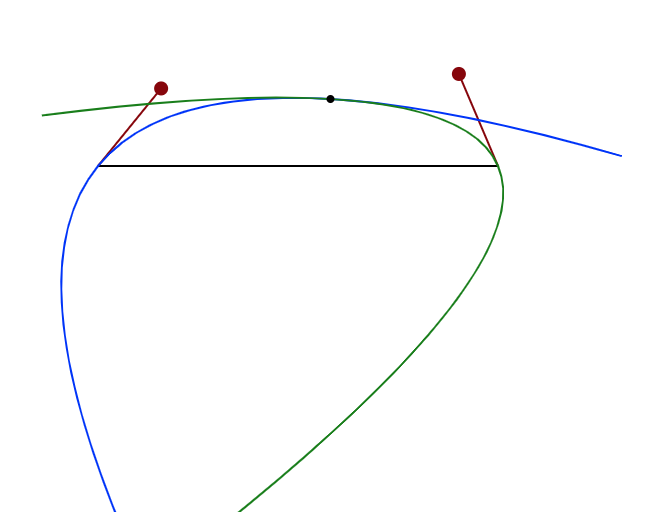
\includegraphics[scale=0.5]{biparabola}
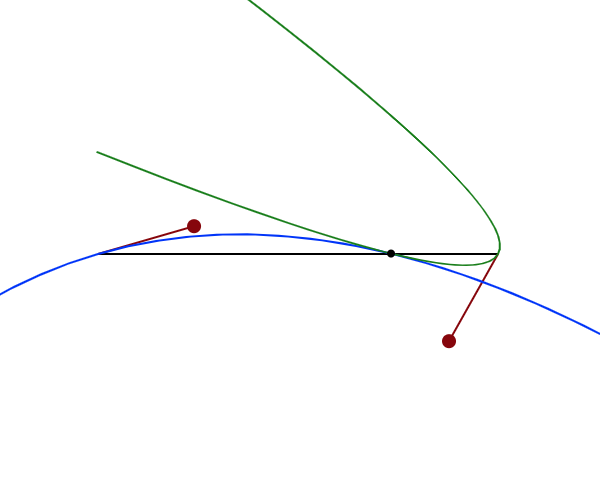
\includegraphics[scale=0.5]{biparabola2}
\caption{Construction of the bi-parabola from tangent constraints}
\label{biparabola}
\end{figure}


This spline has strikingly different properties than the others listed above. It is bounded and is excellently robust. However, it deviates considerably from roundness, and cannot form smooth inflections.

Looking at the curvature map of the bi-parabola curve family reveals a number of fascinating properties. Most notably, the curvature map is periodic in both endpoint tangents, both with period $\pi$. Near a tangent angle of $\pi/2$, the curve forms a \emph{cusp} of infinite curvature, and a reversal of direction. One way or another, the curve has to reverse direction as the tangent goes through its full rotation; with bounded curvature it must flip, so going smoothly through a cusp seems the only other option.

\begin{figure}
\centering
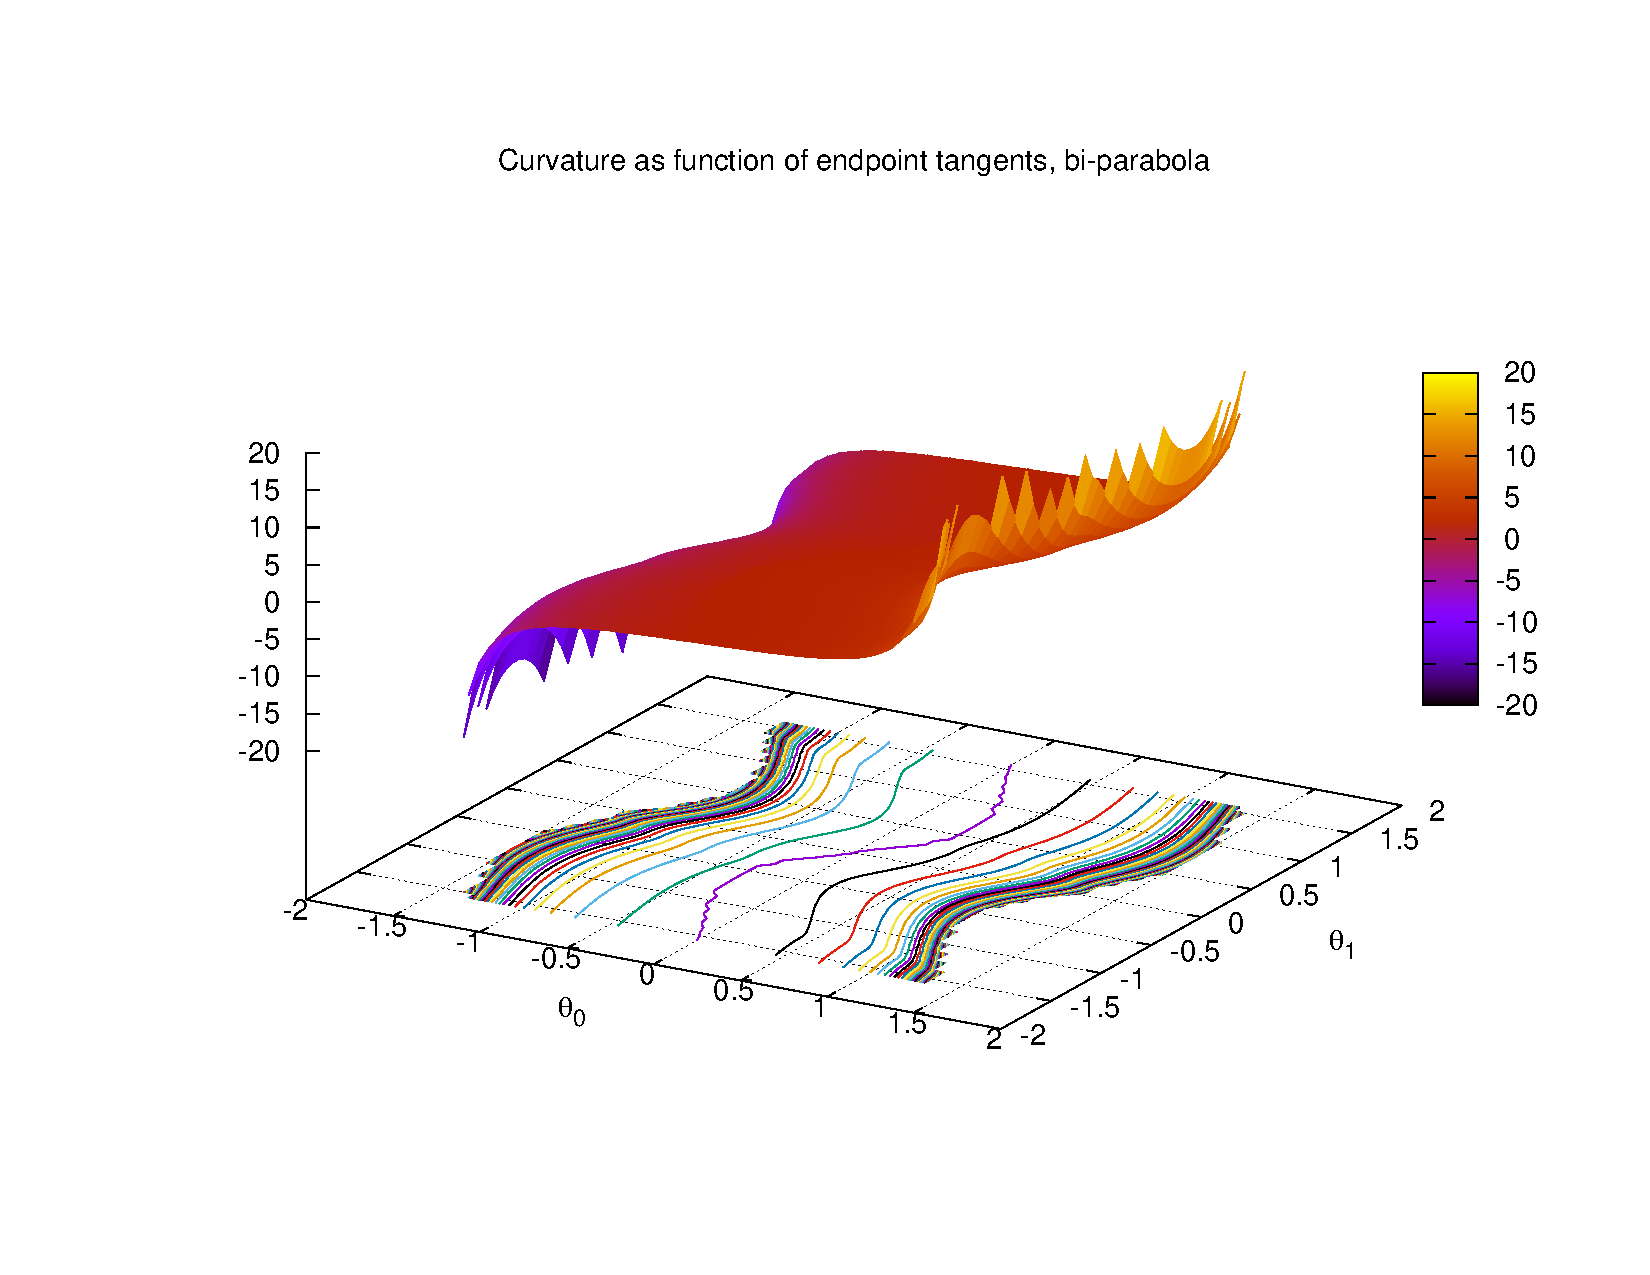
\includegraphics[scale=0.5]{biparab_kmap}
\caption{Curvature map of bi-parabola}
\label{biparab_kmap}
\end{figure}

The \kcurve{} is not extensible, and deviation from roundness is high. It is not monotone curvature, but preserves half of that property - no curvature \emph{maxima} are allowed, while curvature minima are not only allowed but mandatory in the non-inflectional case.

\subsection{Variations on the 2-parameter framework}

Not all interesting splines fall squarely into the 2-parameter paradigm. This section touches on a number of variations.

Perhaps one of the most relevant is the Hobby spline \cite{Hobby85}, which can be seen as an approximation of the Euler spiral spline, particularly at small angles. It is based on a 2-parameter family of curves (at least, ignorning the optional tension parameter) but does not use G2 continuity to determine the endpoints. Instead, it enforces continuity of ``mock curvature,'' a linear approximation of curvature. It has the advantages of robustness and boundedness, at the cost of roundness and extensibility. It is used as the basis for curve design in Apple's iWork products.

Likewise, Ikarus \cite{Karow87} uses a 2-parameter family of curves (biarcs) but uses another scheme to determine the tangent parameters.

A 4-parameter scheme produces splines with G4 continuity. Existing 4-parameter splines include Minimum Variation Curvature \cite{Moreton92} and a 4th order polynomial spiral spline (Chapter 7 of my thesis).

\section{A new spline}

This paper proposes a new spline, fairly simple and easy to compute, that combines the robustness of the \kcurve{} spline with the fine qualities of the Euler spiral spline when the control polygon has low bending angles. In fact, it approximates Euler spiral fairly closely as angles decrease.

First, the formula for the spline is given. As in the Hobby spline, the two-parameter curve family is a single cubic B{\'ezier} segment between each pair of control points. The tangents are given by the parameters.

A cubic B{\'e}zier has two internal control points. Both must lie on the line tangent to the corresponding endpoint, in order to enforce the given tangent constraint. That leaves merely the length the control arm (the signed distance from the endpoint to the control point along the tangent vector) as a free parameter. The new spline uses this simple function for the left control arm length, as a function of $\theta_0$ and $\theta_1$; the right arm is symmetrical:

\[
\begin{aligned}
\mbox{arm length} & = \tfrac{5}{12}(\sin \theta_a - 0.2\sin 3\theta_a), \quad \mbox{\emph{where}} \\
\theta_a & = \theta_0 - 0.3 \sin (2\theta_1 - 0.4\sin 2\theta_1) \\
\end{aligned}
\]

Then, given this two-parameter curve, use a global solver to choose tangents so that the curvature is matched on both sides of each control point. A Newton-style solver as in my thesis will work, but requires a bit more care to make sure that both direction and curvature match, given the possibility of reversals. It also has to cope with curvature being unbounded, as opposed to the bounded curvature of previously published two parameter splines.

For small angles, this spline is quite similar to the Hobby spline; in fact, both can be seen as small-angle approximations to the Euler spiral. But as angles increase, instead of less accurate and more ``globby'' approximations to the Euler spiral shape, the length of the curve creases, and ultimately forms an infinite curvature cusp; beyond that angle, the direction reverses. Its curvature map is periodic (with period $\pi$ in both tangent angles), and grossly similar in this way to the bi-parabola, and so we expect the spline to have similar robustness as the \kcurve spline.

Because it approximates the Euler spiral, the new curve easily handles inflection points, with smooth variation of curvature on either side of the inflection. The new spline has three important elements, which together make it have the desired properties:

\begin{itemize}

\item It is a two-parameter spline with G2 continuity at the control points.

\item The curvature map is periodic, with cusps formed at high angles.

\item The curve family smoothly transitions through zero-curvature inflection points.

\end{itemize}

The curvature map is shown in Figure \ref{newcurve_kmap}.

\begin{figure}
\centering
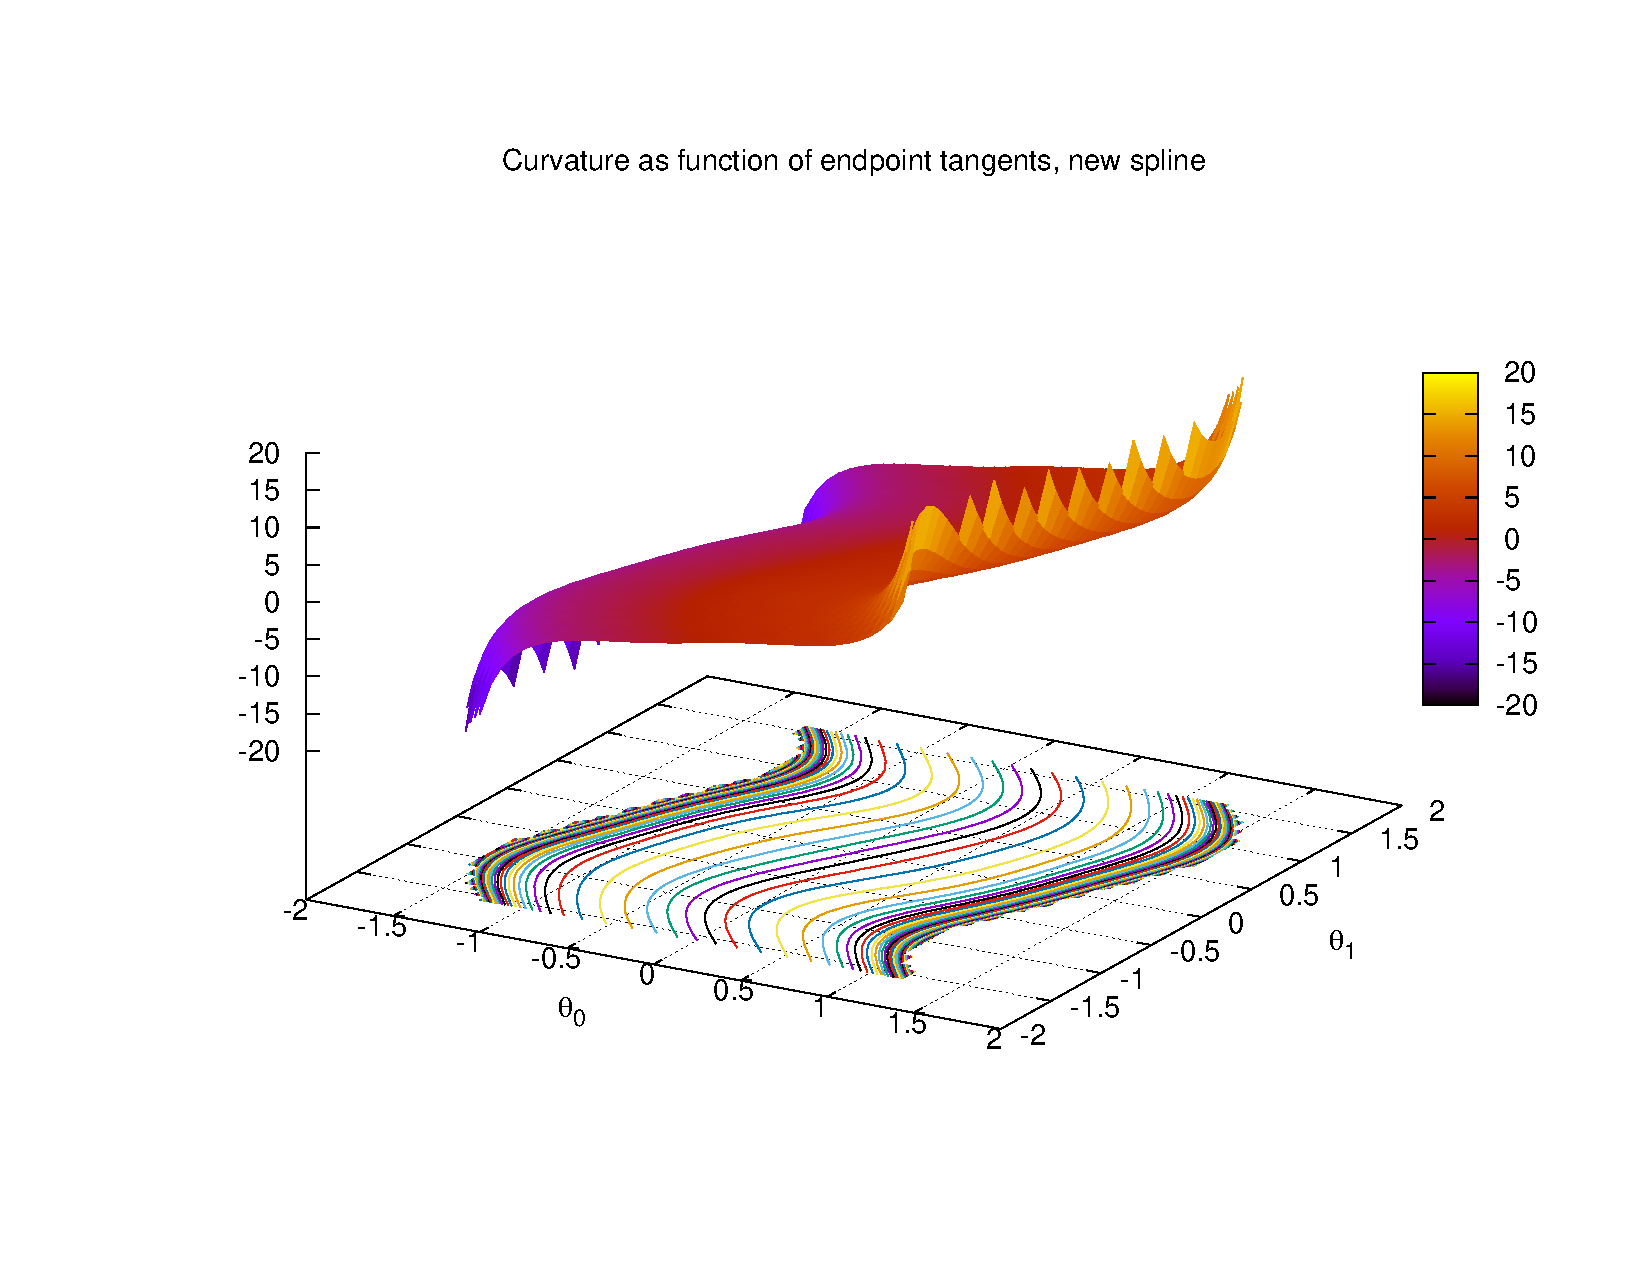
\includegraphics[scale=0.5]{newcurve_kmap}
\caption{Curvature map of new spline curve family}
\label{newcurve_kmap}
\end{figure}

Three families of curves are shown in the following figure, the Euler spiral in red, the bi-parabola in green, and the new curve in blue. The horizontal axis is the left tangent angle, and vertical is the right tangent angle, both in 15 degree increments.

\begin{figure}
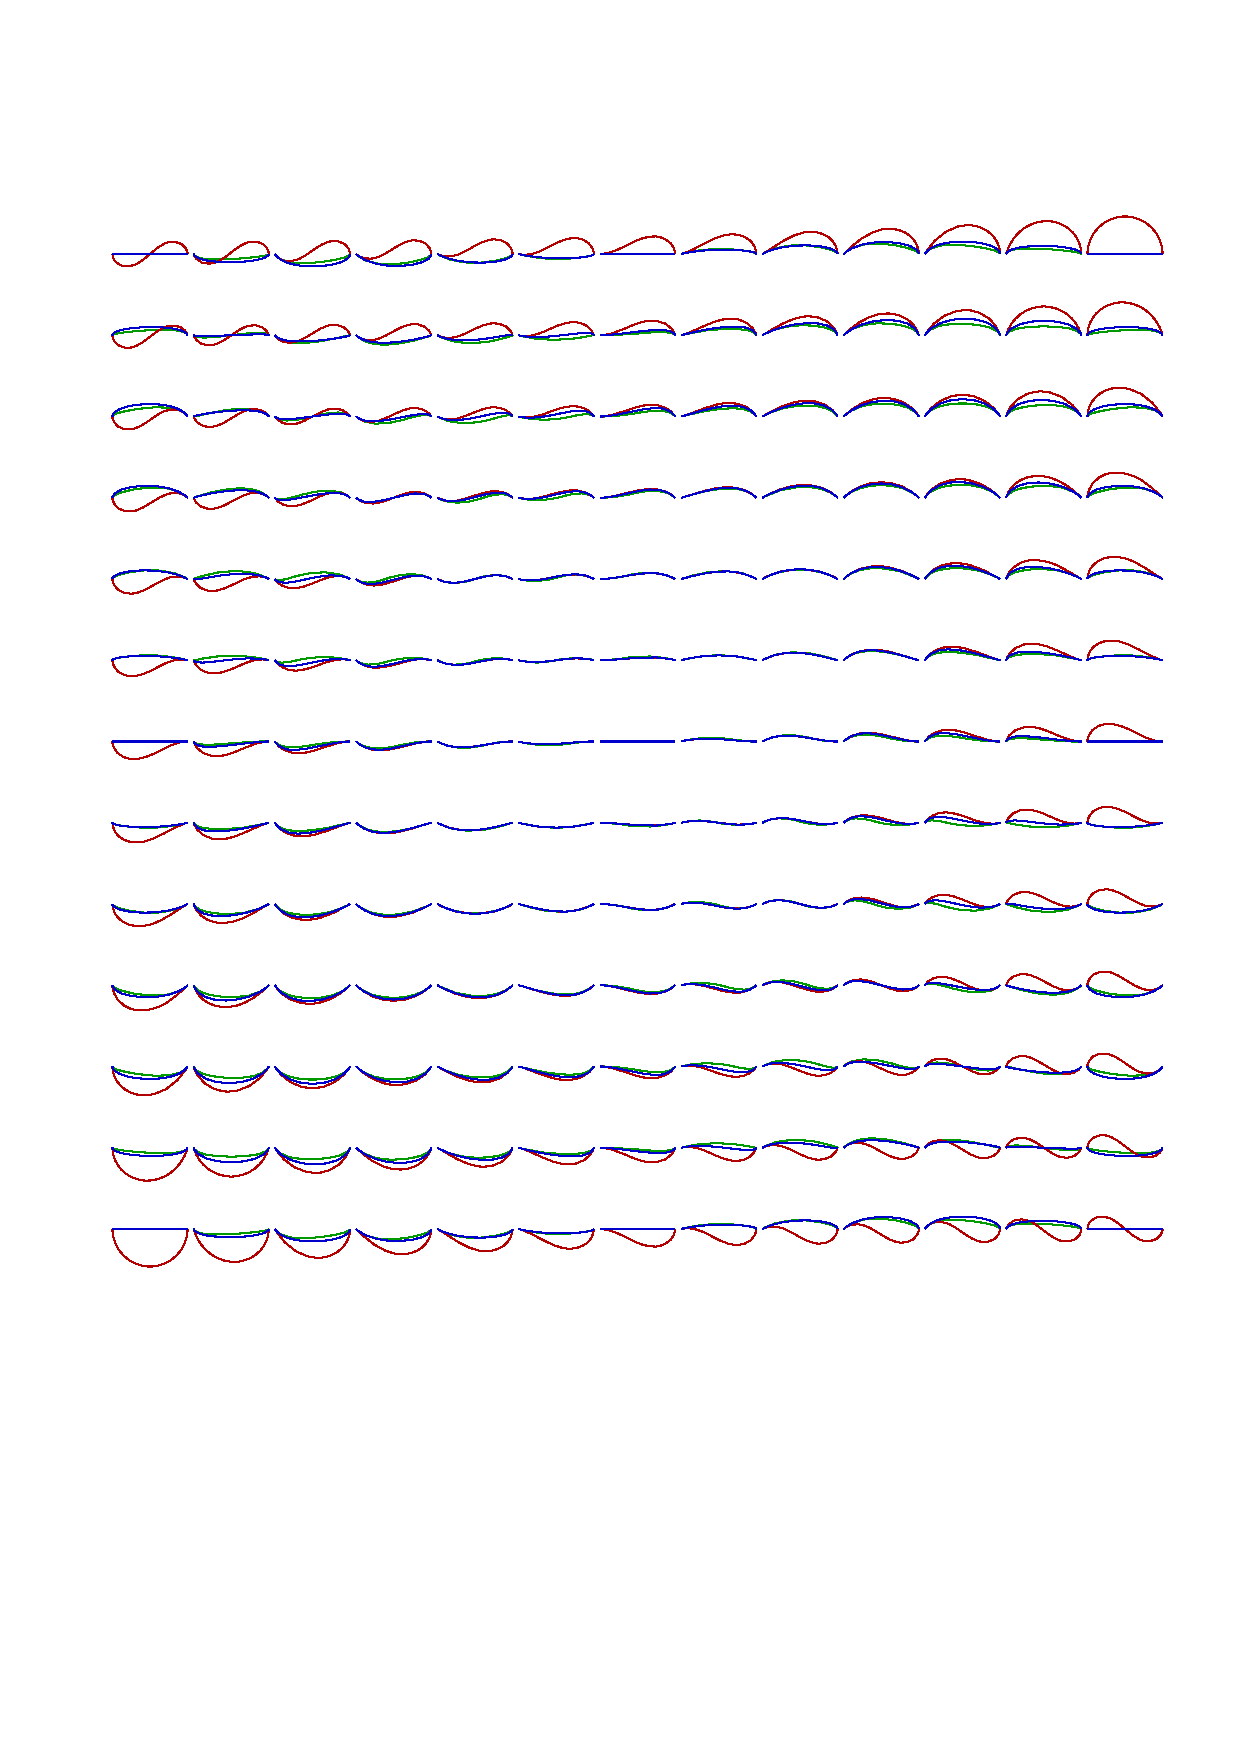
\includegraphics[scale=0.7]{biparab_euler_mycurve}
\caption{Bi-parabola is green, Euler spiral is red, new curve is blue}
\end{figure}

\subsection{Endpoint tangents}

In a cyclic configuration, enforcing G2 continuity across control points discharges all parameters. However, in an open curve, the tangents at the endpoints are unconstrained. These could be explicitly set (for example, in a graphical user interface), but failing that, the spline can set values that make the resulting curve look natural.

It is easiest to set the tangent at the endpoint as a function of the tangent (relative to chord) of the next control point. For example, setting it equal (as in the Euler spiral) sets the terminal segments to circular arcs (as the Euler spiral spline is round and thus generates circular arcs for symmetric tangent constraints). The Minimum Energy Curve sets the endpoint tangents to solve for zero curvature, as this minimizes total bending energy.

A $\pi$-periodic spline has an additional consideration, if it is to be robust -- when the next-to-terminal tangent is $\pi/2$, the terminal tangent should be $0$. This allows the curve to pass smoothly through $\pi/2$ to the other side without a visible ``jump'' to the curve.

The \kcurve{} spline sets the endpoint tangent to $\arctan{2\tan \theta} - \theta$, which solves for a single parabola. We find that $0.5\sin 2\theta$ produces nice results, a bit more curvature than a parabola but less than a circular arc, approximating a circular arc at low angles, and going to $0$ when the opposing tangent is $\pi/2$ for smoothness. Others may prefer a different formula, however.

\subsection{Comparison with \kcurve{}}

Figures \ref{spiral} and \ref{cshape} show a comparison of the new spline with \kcurve{} splines. The first is a simple series of points arranged in a spiral, and shows that the new spline is a much smoother interpolation. The \kcurve{} shows the underlying control polygon too strongly, with prominent curvature maxima.

Perhaps more worrying, Figure \ref{cshape} shows additional pseudo-inflection points added by \kcurve{} for a straightforward ``C'' shape as might be commonly drawn in a font. These curvature reversals are caused by the fact the bi-parabola is not only incapable of forming a true inflection, it also does not have in its repertoire a curve that approaches inflection, with moderate curvature on one end and much lower curvature on the other. The Euler spiral very easily attains such a curve, and the new spline has very similar behavior.

\begin{figure}
\centering
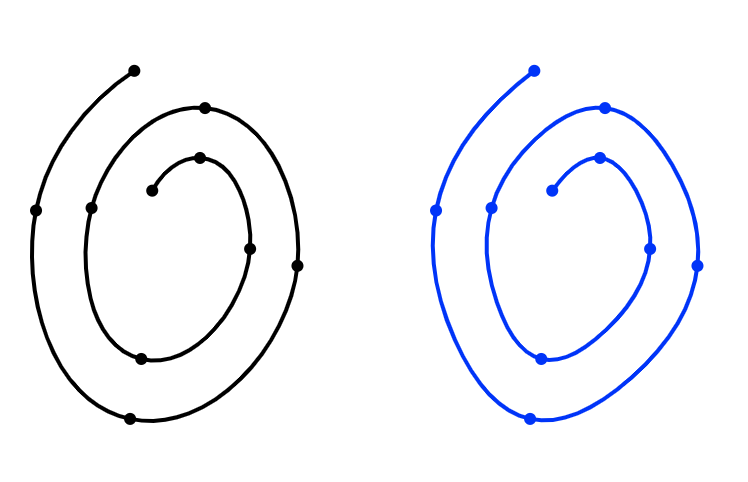
\includegraphics[scale=0.5]{biparab_mine_spiral}
\caption{New spline on the left{}, \kcurve{} on the right, spiral figure}
\label{spiral}
\end{figure}

\begin{figure}
\centering
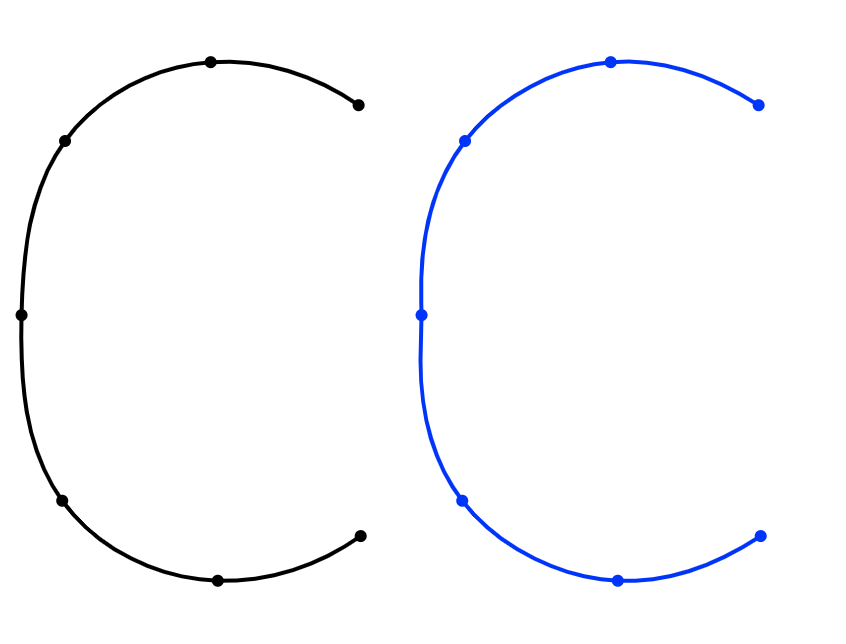
\includegraphics[scale=0.5]{biparab_mine_c}
\caption{New spline on the left{}, \kcurve{} on the right, C shape}
\label{cshape}
\end{figure}

The new spline is not curvature monotonic in the general case. Neither does it exactly respect the property (held by \kcurve) of no internal curvature maxima. However, deviation from this principle is small, and it is easy to imagine a refined version, probably based on more than a single cubic B{\'e}zier per segment, that does.

For inputs containing no large bending angles, the new spline produces results that approximate the Euler spiral, and for this limited class of inputs, the spline approximately has its properties, including roundness, extensionality, and monotone curvature. A refined version of the spline might exactly match the Euler spiral within a certain parameter envelope.

\section{Acknowledgments}

Thanks to Jacob Rus and Carlo S{\'e}quin for discussions providing much insight into the analysis and design of splines.

\section{Bibliography}

\bibliography{paper}{}
\bibliographystyle{plain}

\end{document}
